\chapter{Literature Review}
\label{ch:lit-review}

This thesis seeks to investigate Yolngu seasons from two main perspectives:
a cross-cultural, qualitative exploration of Indigenous knowledge; and
numerical definition and analysis based on this exploration.
%
The literature review first gives a general
overview of the literature on Indigenous Knowledge and methods for respectful
research with Indigenous people.  The second section describes a scientific
understanding of monsoon systems and tropical seasonality, along with previous
approaches to quantitatively describing seasons based on weather events.
The third and final section covers previous research on Indigenous seasons in northern
Australia, and identifies a gap in the literature that this thesis aims to fill.


\section{Indigenous Knowledge}
\label{sec:lit-iek}

There is growing recognition among ecologists, natural resource managers, and
scholars worldwide that Indigenous peoples hold important knowledge about the
natural environment \citep[see eg.][and many others]{clarke2009,prober2011,ens2014}.
The literature on Indigenous knowledge
is well-established and vibrant, across a wide range of topics.
\citet{berkes2012} defines Indigenous Ecological Knowledge as ``a cumulative
body of knowledge, practice and belief, evolving by adaptive processes and
handed down through generations by cultural transmission''.
%
Indigenous knowledge systems not related to ecology are also widely recognised in this literature,
and described by a variety of terms:  \citet{clarke2009} refers to `land-based
knowledge', \citet{petheram2010} and \citet{turner2009} use `traditional
ecological knowledge', while \citet{cochran2015} simply use `indigenous
knowledge'.  This thesis uses the term `Indigenous knowledge', following the
letter of invitation for this research (\cref{app:invitation-letter}, on page~\pageref{app:invitation-letter}) and
emphasising that ecology is not the only subject of Indigenous knowledge.


\citet{turner2009} distinguish Indigenous knowledge systems from `objective'
scientific knowledge on the basis that Indigenous knowledge of practical
matters is value-laden and observations or experience are tangled with beliefs,
philosophy, law, and spirituality.  \citet{woodward2012b}, working in northern
Australia, describes Indigenous seasonal knowledge systems as having strong connections
to ecological knowledge, weather knowledge, resource collection, and spirituality.

In Australia and around the world, Indigenous knowledge is recognised
in areas as diverse as climate change and sustainability assessment
\citep[eg.][]{cochran2015}, holistic fire management \citep[eg.][]{clarke2009,price2012},
customary economic activities including aquaculture \citep{woodward2012a}, and
natural resource management \citep[eg.][]{prober2011}.  The \textit{Environment
Protection and Biodiversity Conservation Act 1999} suggests taking `a
partnership approach to environmental protection and biodiversity conservation'
\citep{ens2012}, which is increasingly common at local and state levels.


Just as written records can be used to construct records of historical weather
events \citep[eg.][]{rodrigo1999}, Indigenous knowledge can improve western
scientific understanding of seasons and climate -- as demonstrated by
\citet{green2010a,clarke2009}, and others (though \citet{green2010a} found
participants attribute recent `strange changes' to local environmental damage
rather than climate change).
%
Observations and knowledge are passed down for generations, forming a
tradition of incredibly detailed understanding at very fine scales \citep{barber2005}.
This unsurpassed detail and nuance makes Indigenous Knowledge highly valuable
in land, environment, and natural resource management applications.
The literature provides a rich context for synthesis of Indigenous Knowledge
and western climate science to investigate Australian seasonality.


There are real challenges involved in cross-cultural research with
Indigenous people.  Individuals and institutions may find it difficult to
invest time and resources in building relationships which may not acheive
existing research goal.  For example, when \citet{petheram2010}
investigated perspectives on climate change adaptation in NE Arnhem Land,
the community instead discussed housing, drugs, and land degradation -- issues
that are crucial to general as well as climate change resilience.

Respectful and appropriate processes are absolutely essential to research with Indigenous communities,
following a long history of dissapointment.  \citet{smith1999} writes that ``the term
`research' is inextricably linked to European imperialism and colonialism ...
one of the dirtiest words in the Indigenous world's vocabulary''. This
connection is practical as well as theoretical.  \citet{woodward2010} notes
that ``the way research agencies engage with Indigenous knowledge authorities
creates a legacy for the next researchers who arrive'', and that community
engagement had been made more difficult by previous researchers who failed to
follow through.

One form of good process for research with Indigneous people is `two-ways'
research, which has seen growing interest internationally and in Australia
\citep{turner2009,prober2011}.  Two-ways research ``uses combinations of
Indigenous and non-Indigenous knowledge and methods, and with the involvement
of both Indigenous and non-Indigenous people towards a common goal''
\citep{ens2014}.
%
\citet{marika2009} offer Yolngu perspectives and metaphors for good process
and governance involving Yolngu and non-Indigenous people , standing in sharp
contrast with the 2007 `Intervention'.  They make the point that Yolngu have
had to adopt or recognise many aspects of non-Yolngu law and culture, and
criticise the failure of non-Indigenous governments to reciprocate.


The research reported in this thesis is situated largely in the two-ways tradition,
as a natural continuation of pre-existing collegiate relationships between
the author and several participants.  Without the
trust and respect built over years in these relationships, and the opportunity
to follow up outside of academic deadlines, a good process for this study
may have been impossible.



\section{The Tropical Climate and Seasons}
\label{sec:lit-tropical-climate}

This section presents a short introduction to the quantitative scientific
perspective on the tropical climate and seasons, covering the large-scale
drivers of the seasons, detection of monsoon onset, and previous
weather-based season definitions in northern Australia.
%
Tropical climates and seasons are driven by three global patterns of
atmospheric circulation:  the Hadley cells of the general circulation of
the atmosphere, the Coriolis effect, and the axial tilt of the Earth.

Hadley cells are a feature of the global atmospheric circulation
caused by the variation in insolation (solar energy delivered per unit area)
by latitude, which is greatest at the equator.  As the warm air rises and
cools, rain condenses out and forms the distinctive wet band of the tropics
before air spreads towards the poles at high altitude.
Air at the surface tends to move towards the \textit{inter-tropical
convergence zone} (ITCZ), causing the trade winds when deflected east or west
by the Coriolis effect (\cref{fig:itcz-india-aus}) \citep{kump2010}.
The mid-latitude and polar cells shape climates at higher
latitudes, but are not directly relevant to tropical seasonality.

Monsoon seasonality can be understood as the ITCZ moving north or south
with the latitude of greatest insolation, which changes due to the
axial tilt of the Earth as it orbits the sun.  While this is strongly
associated with rainfall, the fundamental indicator is the direction of
the prevailing wind: generally south-easterly below the ITCZ, and generally
north-westerly above \citep{kump2010}.  \Cref{fig:itcz-india-aus} shows how this pattern
manifests in reversed seasons between India and Northern Australia.
The presence of the ITCZ is associated with the Wet season and greatest
rainfall, and its absence with the Dry season \citep{sturman2005}.

\begin{figure}[p]
    \centering
    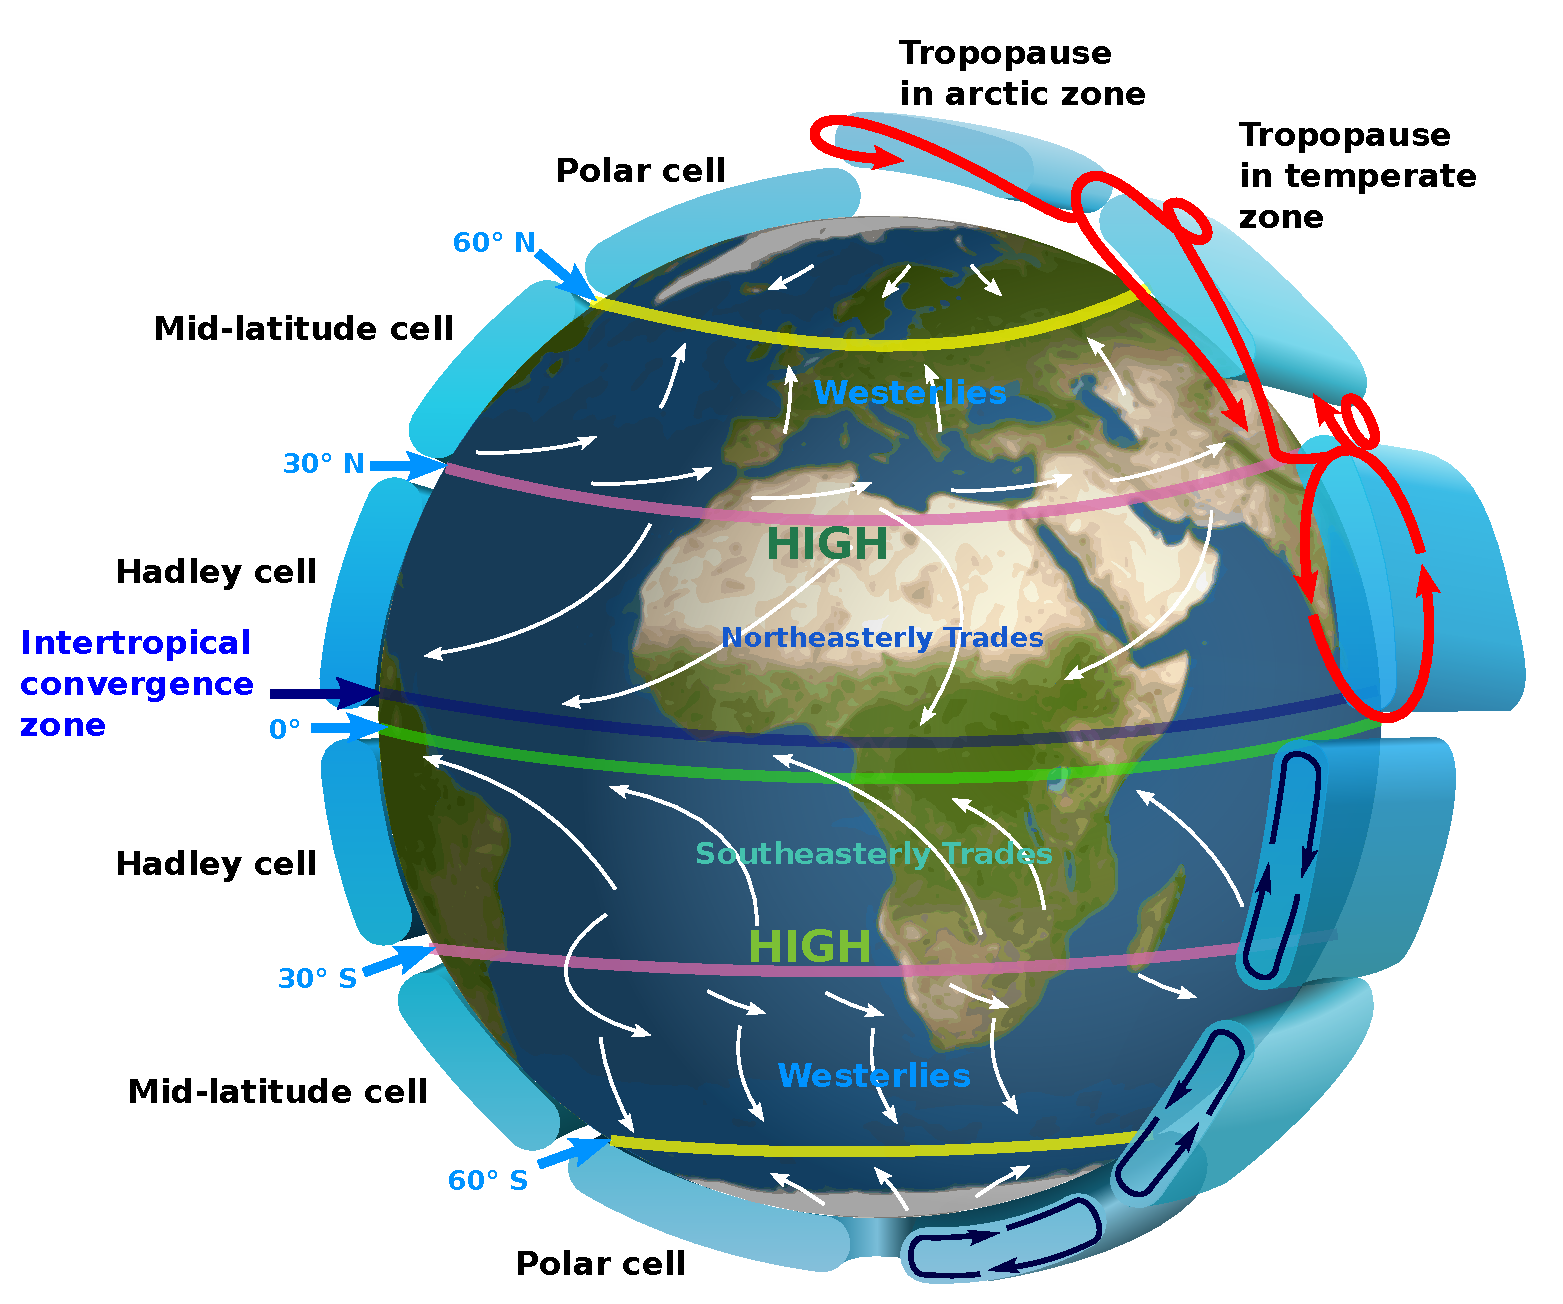
\includegraphics[width=0.8\linewidth]{Earth_Global_Circulation.pdf}
    \caption[Hadley Cells and trade-winds]{
        Diagram showing surface-level prevailing winds (white arrows),
        Hadley Cells, and the Intertropical convergence zone (`ITCZ').
        Air rises at the ITCZ, heated by the highest - intensity sunlight.
        This causes a low-pressure band of trpoical rainfall, and the
        trade winds -- deflected towards the west by the Coriolis Effect.
        \citep[image:][]{kaidor2013}
        }
    \label{fig:hadley-cells}
\vspace{1cm}
    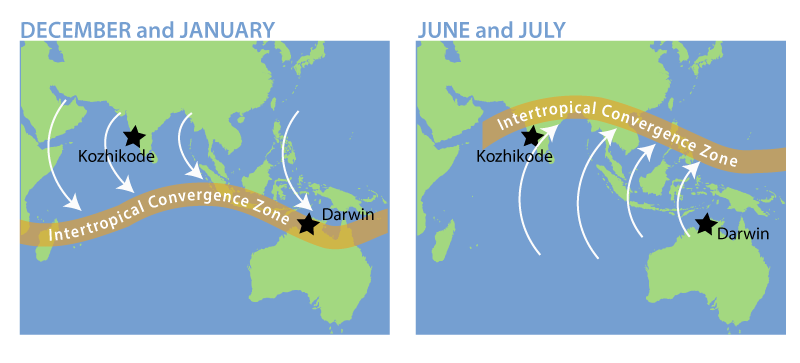
\includegraphics[width=0.8\linewidth]{itcz.png}
    \caption[ITCZ showing northern and southern monsoon]{
        Approximate location of the inter-tropical convergence zone
        (yellow band) during the northern and southern monsoon.
        White arrows show prevailing wind direction; rainfall is
        associated with the ITCZ.  \citep[image:][]{boos2014}}
    \label{fig:itcz-india-aus}
\end{figure}

At a local scale, a monsoonal cycle is often described with `Wet' and
`Dry' seasons, sometimes with a separate pre-wet 'buildup' \citep{kingsley2003}.
In the Northern Territory of Australia both are warm to hot, with distinctive
changes in humidity and wind direction.  The characteristic pattern of tropical
seasons -- distinct hot/wet and cooler/dry periods -- is clearly visible in
monthly averages of temperature and rainfall, which are given for the study
area in \cref{tab:galiwinku-monthly-summary,fig:galiwinku-climograph}.
Note that the more nuanced patterns described by Indigenous seasons are not
visible in these summaries; \cref{ch:results} shows that this level of detail
requires analysis of daily observations.


Monsoon onset is quantitatively characterised using a variety of approaches.
\citet{sultan2003,fasullo2002}, and \citet{wu1998} use wide-scale definitions
-- based on moisture transport, rainfall, and regional climate indicies.
\citet{hendon1990}, using observational data from a single station, base their
analysis on prevailing high-altitude wind.  Each of these definitions use a
locally appropriate proxy for the state of the ITCZ,
which is the ultimate driver of monsoon seasonality.

\defcitealias{SMHI2015}{SMHI 2015}

There is a considerable body of literature dealing with seasons defined
by observed environmental change -- from temperature thresholds in Sweden
\citepalias{SMHI2015} to `leaf out' for botanists \citep[eg.][]{allstadt2015}
or butterflies for zoologists \citep[eg.][]{forister2003,roy2000}.
Indicators which cycle through qualitatively distinct states, such as deciduous
leaves, are relatively accurate and easy to interpret but may be unavailable
in some contexts.

In Australia, \citet{holland1985} considers rainfall-based definitions of the
monsoon, which demonstrate good agreement with definitions based on zonal
wind in the lower troposphere.  He concludes that pre-monsoon
rainfall varies too much between sites (due to local conditions and events)
to serve as a useful definition on a wider scale.
%
However, surface-level station observations may still form a useful basis for
understanding Indigenous calendars, which are non-comparable between sites
for similar reasons.

A slightly different approach to the seasonal cycle of Northern Australia
describes 'dry', 'rainy', and 'wet' seasons, with the wet as a subset of the
longer rainy season.  The dry season is defined as the period where the probability
of no rain for ten days is greater than 50\%.  The rainy season is defined by
the complement (\textless50\% chance of no rain), beginning slightly before the
monsoon (defined by wind) and ending slightly after.  Within the rainy season, the `et season
is defined as having less than a 10\% chance of a ten-day dry spell.
%
\citet{cook2001} develop and justify these definitions based on their close relationship with
ecological patterns, especially spatial patterns in tropical vegetation,
and argue that a proper understanding of tropical seasonality in Northern
Australia must account for rainfall events outside of the monsoon period.



\section{Australian Indigenous Seasons}
\label{sec:aus-indig-seasons}

% Start section, so it fills the first good page instead of leaving a gap
\begin{sidewaysfigure}
    \vspace{0.3in}
    \centerline{ 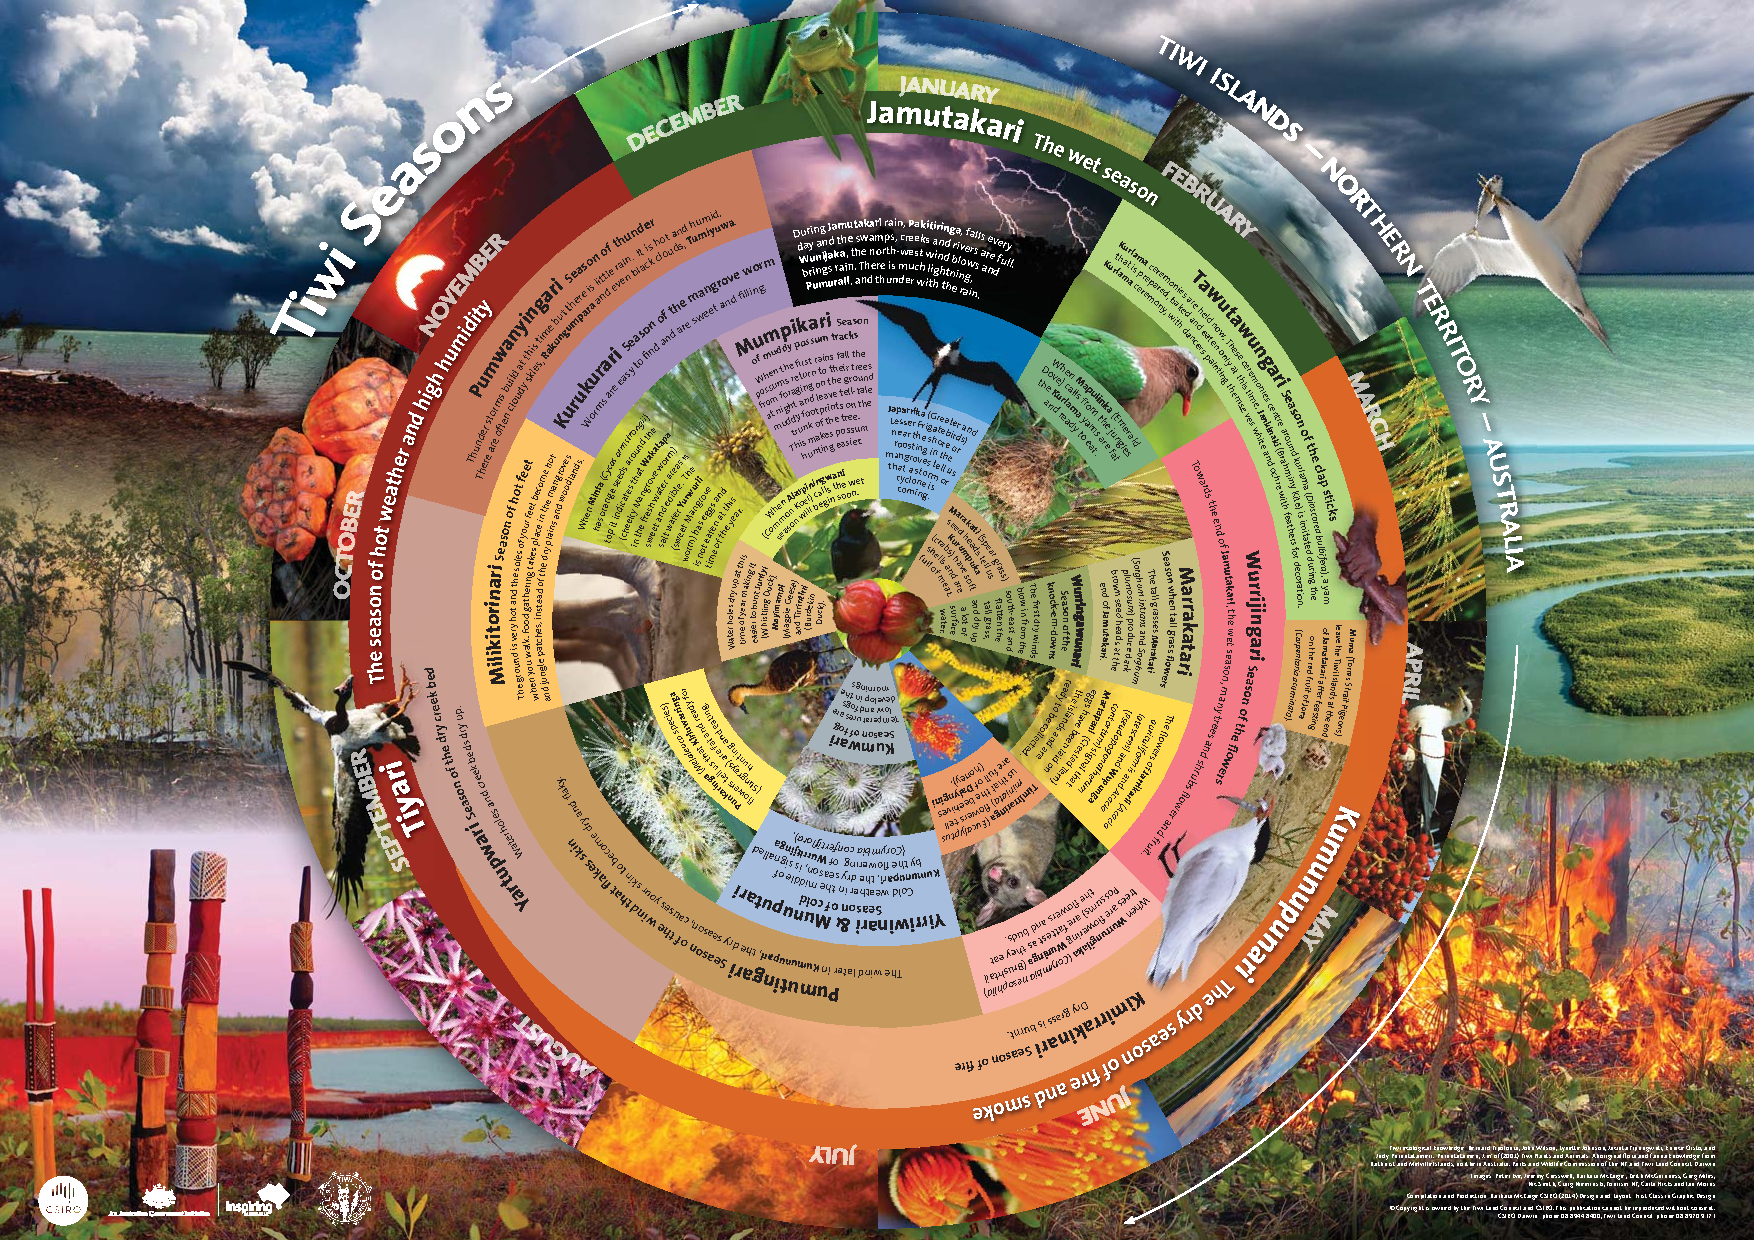
\includegraphics[width=9in]{TiwiSeasonsA4.pdf} }
    \caption[The Tiwi Seasons Calendar \citep{CSIROcals}]{
        The Tiwi Seasons Calendar \citep{CSIROcals}.
        This calendar shows month of year in the outermost ring,
        then three `major' Tiwi seasons recognised by weather.
        Note that \textit{Kumunupunari} does not have a sharp boundary with \textit{Tiyari}!
        Within this ring are smaller seasons, recognised by weather
        or ecological events and associated with particular activities.
        }
    \label{fig:tiwi-seasons}
\end{sidewaysfigure}

% And after the fullpage figure, this should be the bottom of the next page
\begin{SCfigure}[][bth]
    \centering
    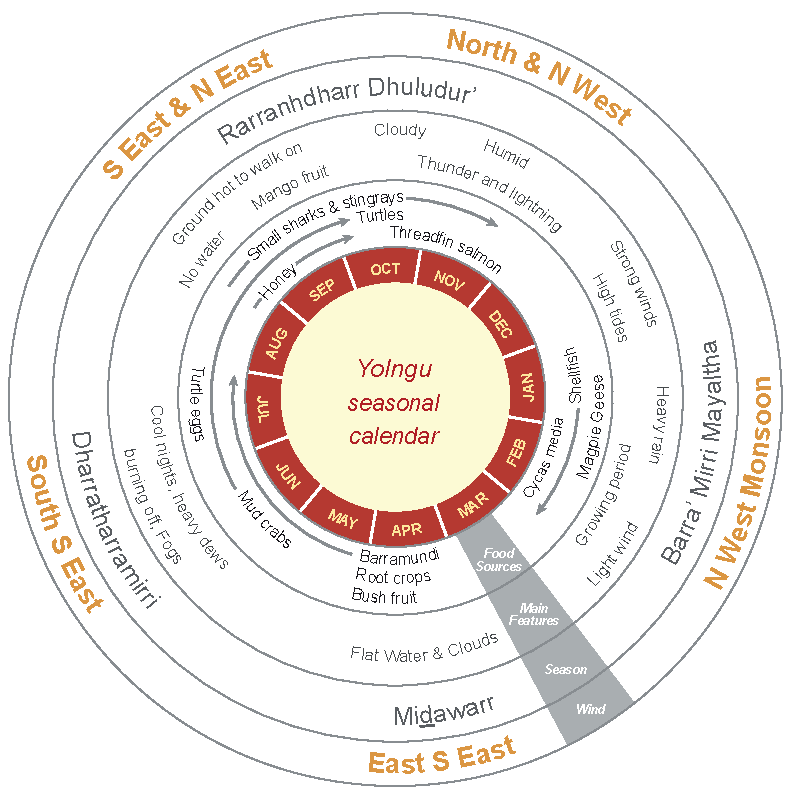
\includegraphics[width=0.7\textwidth]{davis1989_yolngu_seasons.pdf}
    \caption[Yolngu seasonal calendar for Milingimbi \citep{davis1989}]{
        Yolngu seasonal calendar for Milingimbi, redrawn from \citet[p2]{davis1989}.
        This calendar shows a glimpse of the relationships between season,
        prevailing wind, typical conditions, and available foods.
        It also shows typical gregorian months, for non-Indigenous readers.
        \citet[][p.107]{barber2005} draws a similar figure -- also following
        Davis -- for the distinct Yolngu calendar at Blue Mud Bay.
        }
    \label{fig:yolngu-seasons}
\end{SCfigure}


The European seasons of Summer, Autumn, Winter, and Spring are adapted for
agriculture in temperate regions with low inter-annual variability, which
allowed formal definition in terms of date rather than temperature or rainfall.
These seasons begin and end at dates given either by the solstices and equinoxes,
or by Gregorian calendar month.


Australian Indigenous seasonal calendars serve a similar purpose in informing
resource use and management, but manifest in qualitatively different ways.
Instead of date, seasons are defined by weather events and ecological cycles,
with all the sensitivity to local context and variation between years that
this implies in the Australian context \citep{davis1989}.  An enormous volume of ecological and
resource-management knowledge is embedded in these calendars, and passed
down over many generations in complex ways \citep{barber2005}.
%
\citet{woodward2012b} explains that Australian Indigenous seasonal knowledge
consists of four key aspects: ``a focus on resource use, knowledge of complex
ecological indicators to facilitate resource collection, knowledge of
meteorological phenomena and a strong metaphysical/spiritual understanding.''.
This emphasises the nuance and value of Indigenous knowledge of tropical
seasonality, which goes far beyond the Wet/Dry/Buildup cycle recognised
by non-Indigenous locals \citep{kingsley2003}.


Despite the novelty and potential value of combining Indigenous seasonal
knowledge with quantitative climate science, this topic remains a gap
in the Australian literature.  \citet{cochran2015} demonstrate this potential
in assessment of climate monitoring methodology in the Tiquie River basin,
in South America.  Keyword searches in the ANU library collection, Google
Scholar, and a number of publishers did not return any relevant results.
With a relatively short and sparse instrumental record, and little investigation
of proxy records in northern Australia, Indigenous knowledge and oral histories
are a promising avenue for characterisation of historical climates


Previous studies of Yolngu seasons have tended to treat Indigenous Knowledge
as an \emph{object of} academic research; this thesis additionally treats
Yolngu knowledge as a \emph{framework for} research.  These studies have generally
been motivated by academic study, project work by government agencies, or
Indigenous people sharing their knowledge -- in most cases, several of these
factors are at work.  A more useful distinction is therefore between posters
(produced for the Indigenous and general communities), shorter material such
as articles or web-pages, and long-form theses or books.

The best-known representation of Indigenous seasonal calendars in Australia
is the poster series developed by multiple researchers and Indigenous
communities, driven and collated by \citet{CSIROcals}.  This series started with the
Ngan'gi Seasons Calendar in 2009 (on the Daly River, NT) and includes the Tiwi Seasons Calendar
(\cref{fig:tiwi-seasons}).  The process is driven by Indigenous participants
who want to record and share their knowledge to be recognised by all people
\citep{woodward2010,oconnor2010}.  The main focus is ecological knowledge and
customary activities or resource use.  These posters have become a source of
pride for Indigenous people beyond the participating groups; one interview
for this research was relocated to visit a poster display.  \citet{gotha2012}
demonstrates that the value of this process and format is recognised outside
CSIRO; and during fieldwork I saw many more such calendars in the `grey
literature' -- mostly produced for remote-area schools and community centers.


The recent increase in research on Australian Indigenous calendars can be
traced to the 2002 creation of a `Indigenous Weather Knowledge' website by the
\citet{BOM-iwk}, in partnership with Monash University and the Aboriginal and
Torres Strait Islander Commission.  In 2016, the website describes eleven
Indigenous calendars in varing levels of detail, from a simple summary of what
seasons are recognised, to posters produced with CSIRO and accompanying reports.
\citet{kingsley2003} speculated that this might eventually lead
to widespread adoption of local Indigenous calendars, and the trend since is promising.
%
A range of articles and reports have accompanied the CSIRO posters, mostly
focussed on the process \citep[eg.][]{woodward2010,oconnor2010}.  Other
publications have considered Indigenous calendars in the context of
climate change \citep[eg.][]{green2010a,green2010b},
ecological assessment \citep[eg.][]{ens2012,prober2011}, and other topics.
Few document the structure or content of Indigenous knowledge of seasons, with
the notable exception of \citet[eg.][]{woodward2012b}.


The most substantial sources of published information about Yolngu seasonal
knowledge identified in the literature review are \textit{Man of All Seasons}
\citep{davis1989}, and the \textit{Yan-nhangu Atlas and Illustrated Dictionary}
\citep{atlas2014}.  \textit{Where the Clouds Stand}, a PhD thesis by
\citep{barber2005}, is available online and provides a third perspective.
These references cover the content and context of Yolngu seasons and knowledge
in substantial detail, with a strong anthropological focus.
%
\citet{davis1989} writes about the seasons at Milingimbi in detail,
describing the weather, wildlife, and customary activities of each.  The book
draws on his experience as a teacher at Galiwinku, and includes
numerous original photographs.
%
The \textit{Yan-nhangu Atlas} is intended to safeguard the language and
traditional knowledge of the Crocodile Islands (NW of Milingimbi and east
to Galiwinku, see \cref{fig:arnhem-map}).  It has relatively little content
related to seasons -- only a few pages -- but may be regarded as authoritative.
%
\textit{Where the Clouds Stand} is a PhD thesis in Anthropology, drawing on
more than a year living with Yolngu at Blue Mud Bay (aproximately 150 km
south-east of the study area).  Barber highlights the depth and complexity
of Yolngu knowledge, with seasonality playing a pervasive role in everyday
life.  Within the same language group Barber gives a calendar with
seven seasons, of which only three are shared with the study sites for this
thesis.
%
Specific quotations from each are included in here in \textit{\nameref{sec:calendar-description}}
(\cref{sec:calendar-description}), supporting the descriptions of seasons
gathered through fieldwork.

